\chapter*{L´Equateur de Cuenca à Baños\markboth{L´Equateur de Cuenca à Baños}{}}
\section*{22 juin 2015}
Je quitte le Pérou depuis Trujillo en bus vers Cuenca : 4h de bus jusqu´à Chiclayo, suivi d´un bus de nuit vers l´Equateur avec passage de la frontière au milieu de la nuit. \newline
 Cuenca est une jolie ville située a 2500m d´altitude dans la sierra équatorienne. Le climat est frais et le temps très instable comme je vais m´en apercevoir sur la route ensuite. \newline
 \newline
\centerline{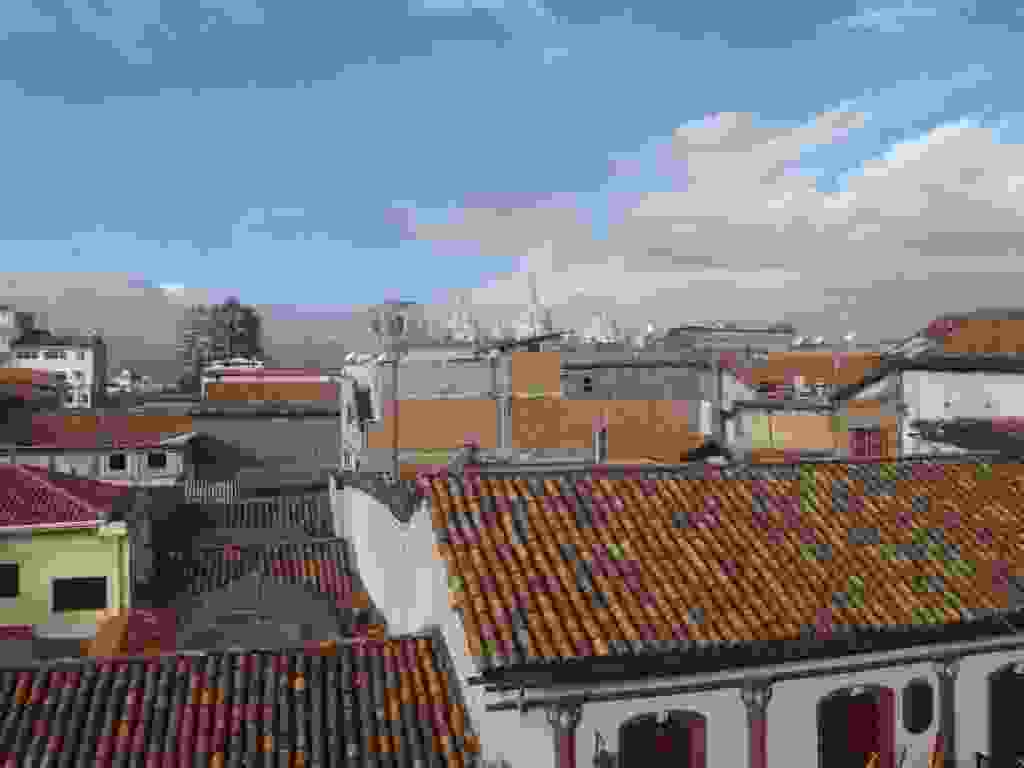
\includegraphics[width=\mywidth]{../wp-content/uploads/2015/06/P6124839-1024x768.jpg} } 
 \newline
 \newline
\centerline{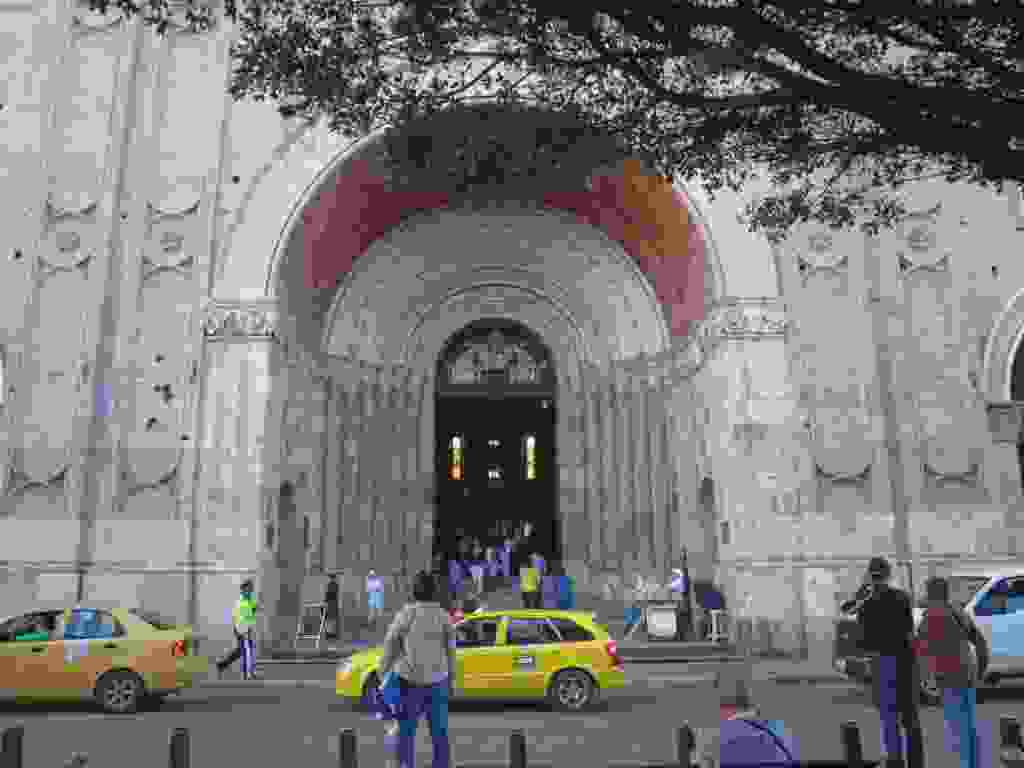
\includegraphics[width=\mywidth]{../wp-content/uploads/2015/06/P6124844-1024x768.jpg} } 
 \newline
 \newline
\centerline{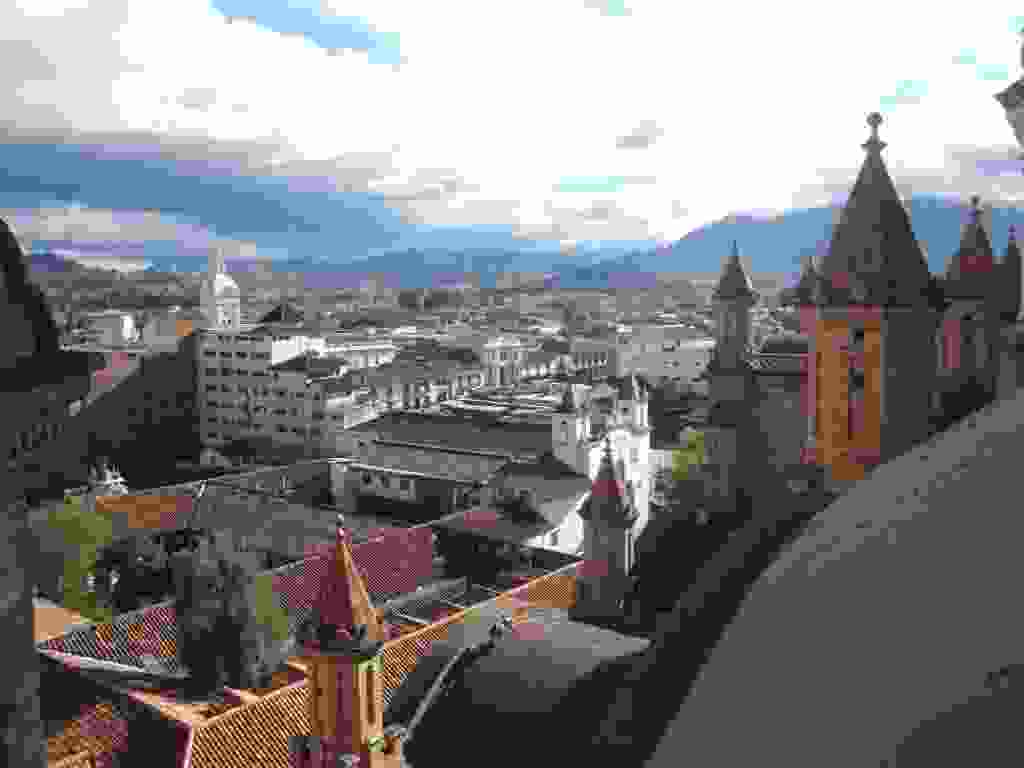
\includegraphics[width=\mywidth]{../wp-content/uploads/2015/06/P6124846-1024x768.jpg} } 
 \newline
 \newline
\centerline{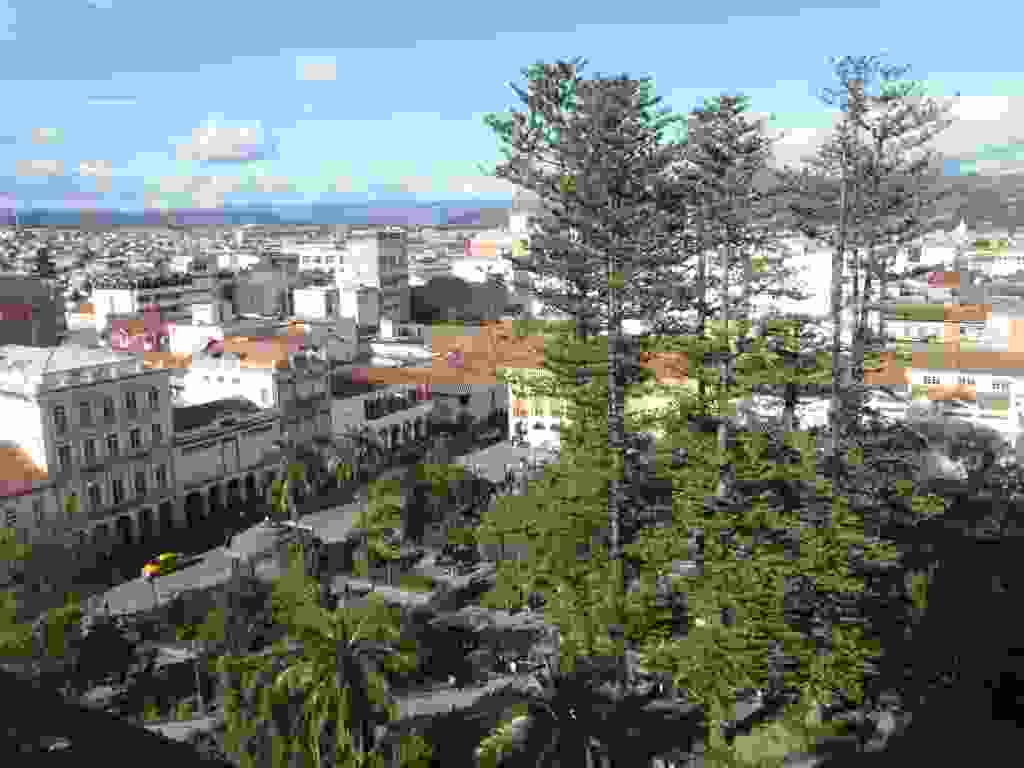
\includegraphics[width=\mywidth]{../wp-content/uploads/2015/06/P6124849-1024x768.jpg} } 
 \newline
 \newline
\centerline{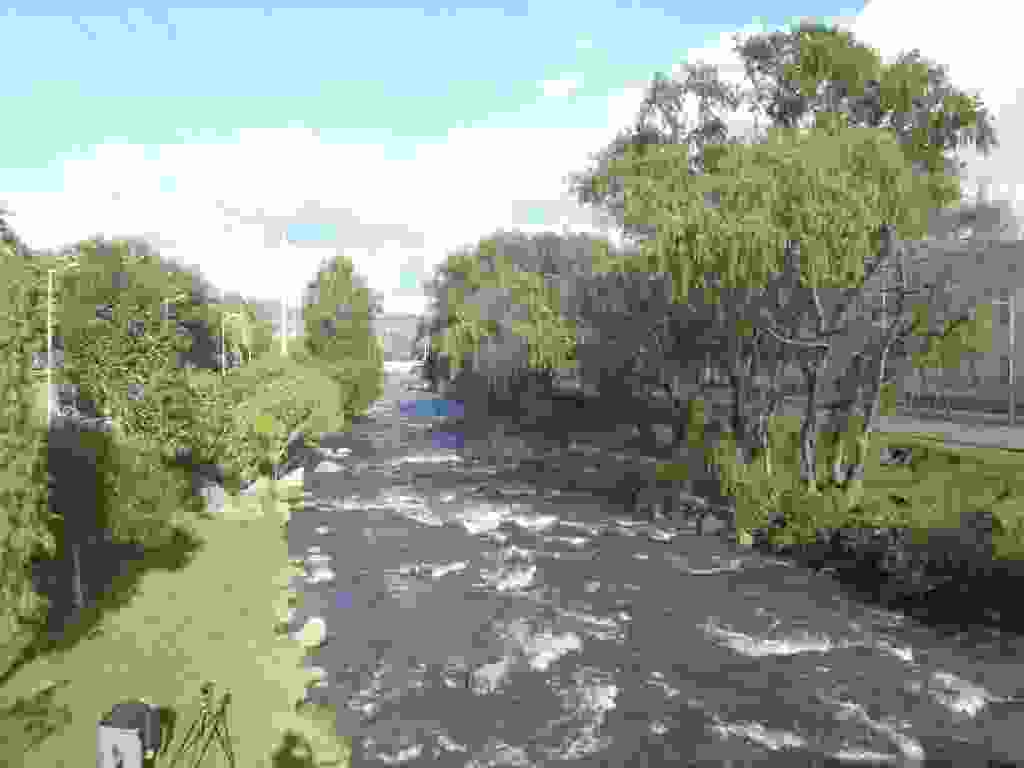
\includegraphics[width=\mywidth]{../wp-content/uploads/2015/06/P6124852-1024x768.jpg} } 
 \newline
 Encore beaucoup de fruits dans les marchés ici. \newline
 \newline
\centerline{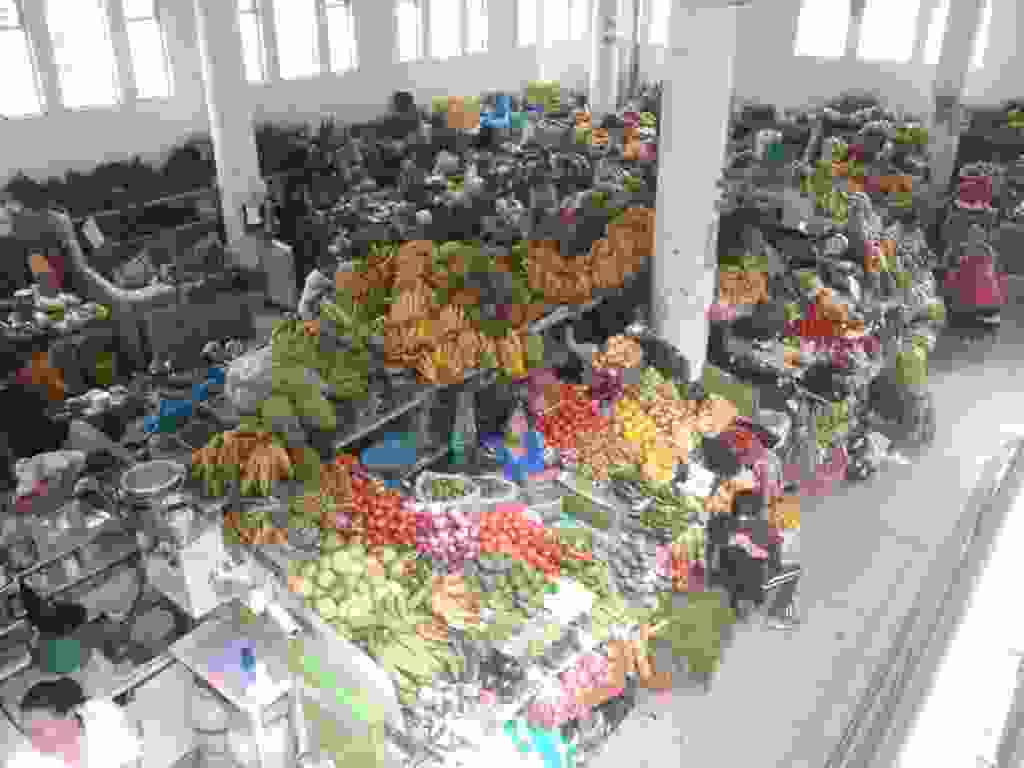
\includegraphics[width=\mywidth]{../wp-content/uploads/2015/06/P6134855-1024x768.jpg} } 
 \newline
 Je visite le musée archéologique. \newline
 \newline
\centerline{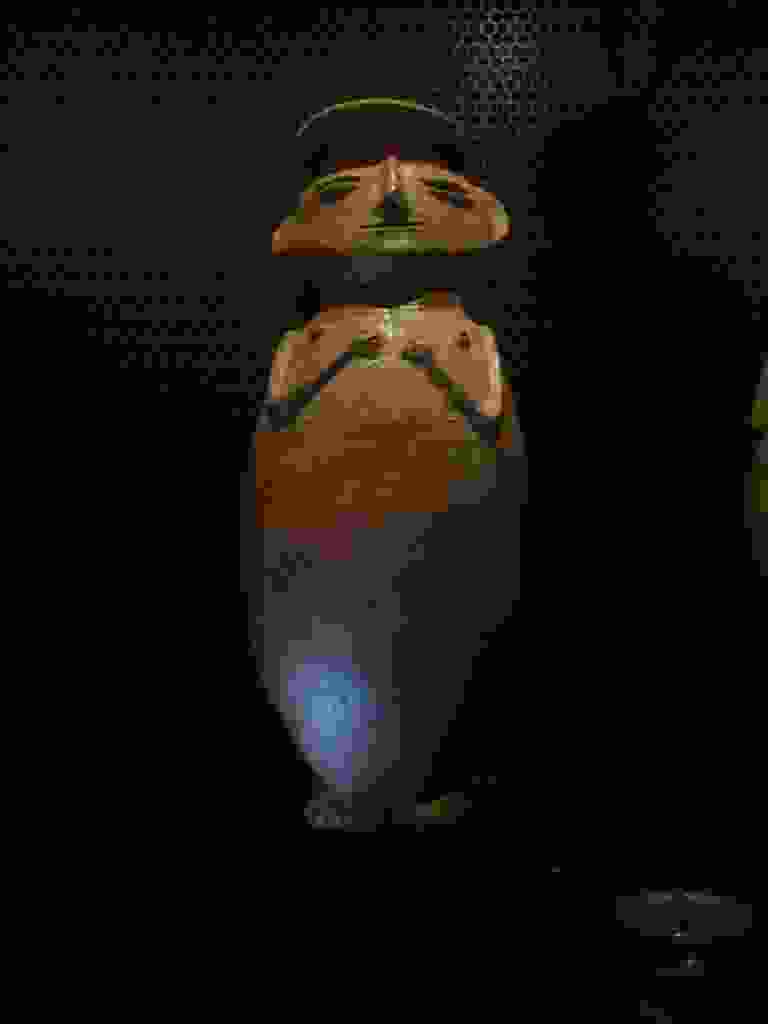
\includegraphics[width=\mywidth]{../wp-content/uploads/2015/06/P6134859-768x1024.jpg} } 
 \newline
 Puis une balade au parc national Cajas près de Cuenca. \newline
 \newline
\centerline{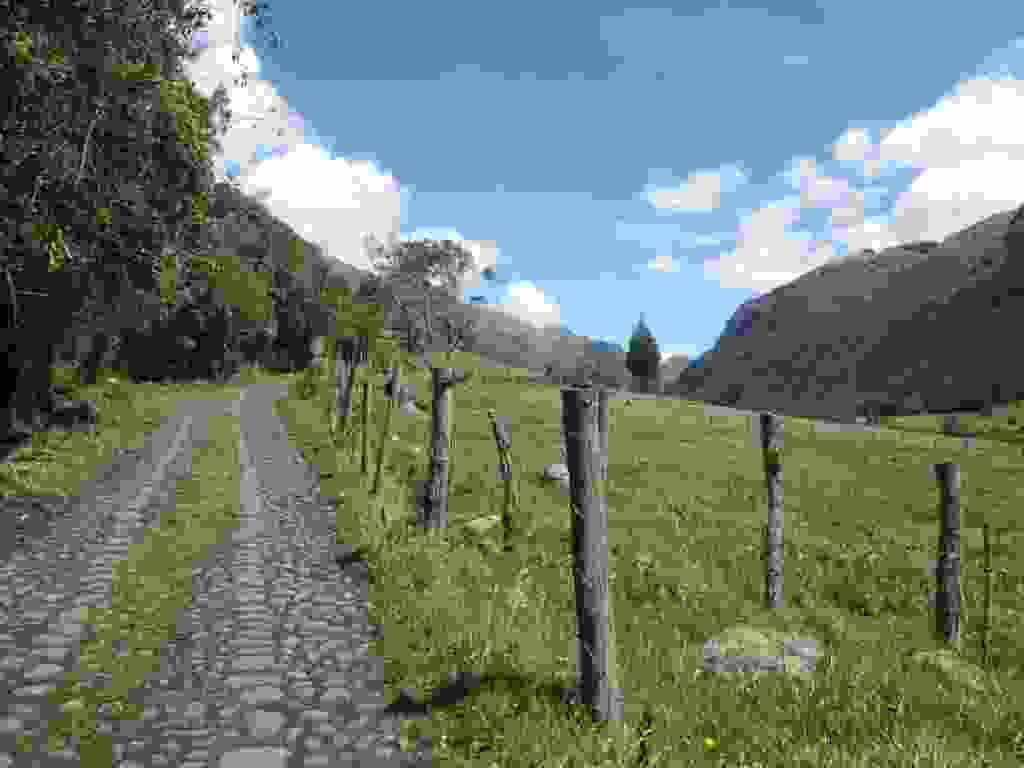
\includegraphics[width=\mywidth]{../wp-content/uploads/2015/06/P6144861-1024x768.jpg} } 
 \newline
 \newline
\centerline{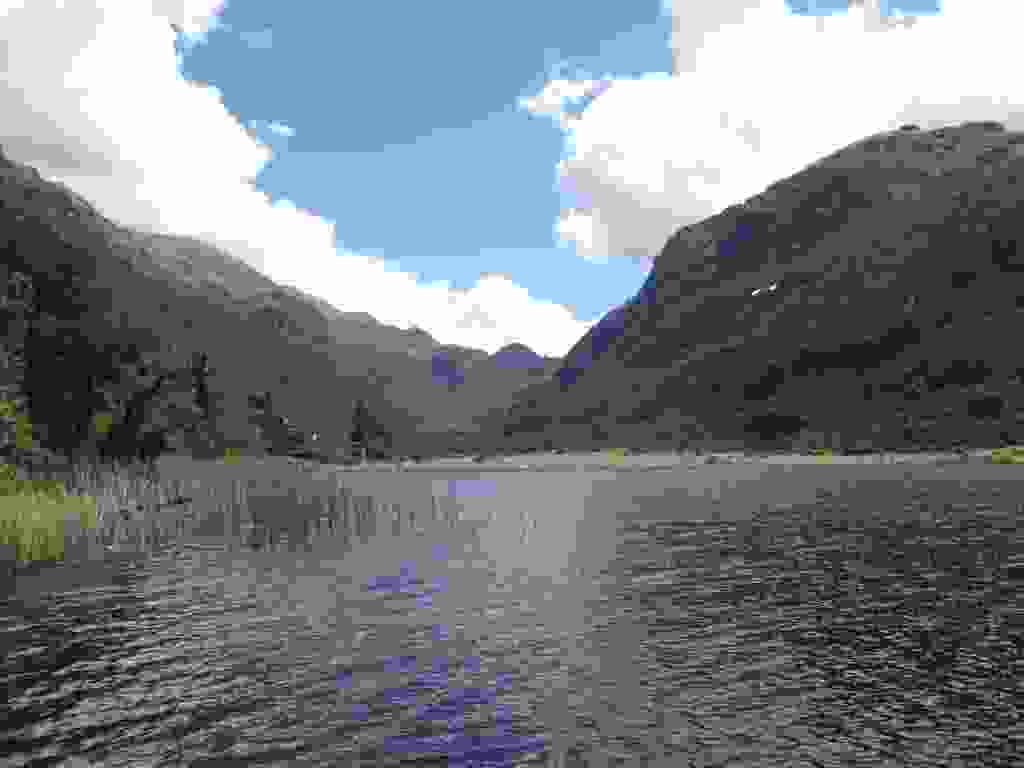
\includegraphics[width=\mywidth]{../wp-content/uploads/2015/06/P6144868-1024x768.jpg} } 
 \newline
 \newline
\centerline{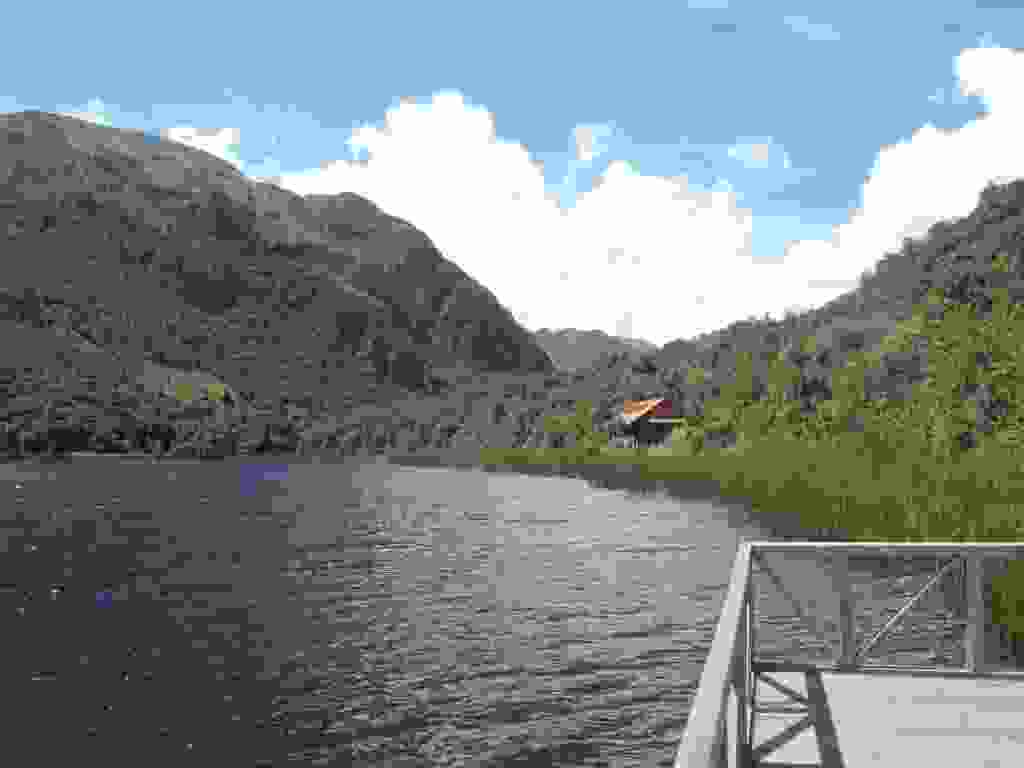
\includegraphics[width=\mywidth]{../wp-content/uploads/2015/06/P6144869-1024x768.jpg} } 
 \newline
 \newline
\centerline{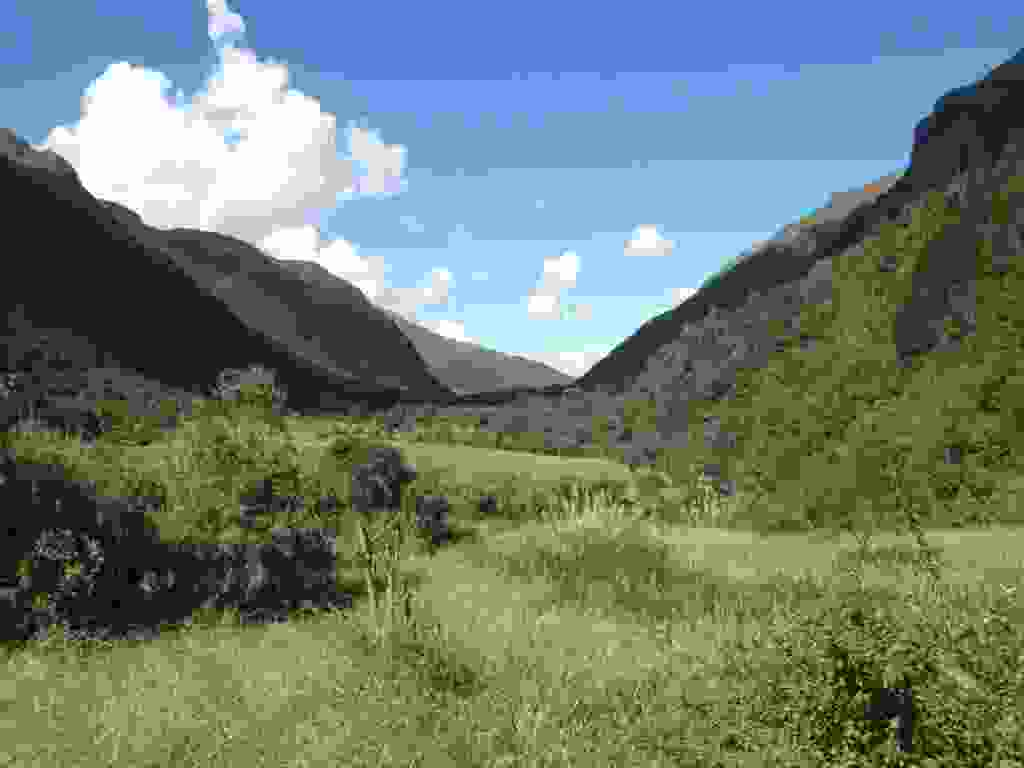
\includegraphics[width=\mywidth]{../wp-content/uploads/2015/06/P6144878-1024x768.jpg} } 
 \newline
 J´avais prévu de camper une nuit dans le parc mais l´état du chemin me fait faire demi-tour et rentrer à Cuenca. \newline
 \newline
\centerline{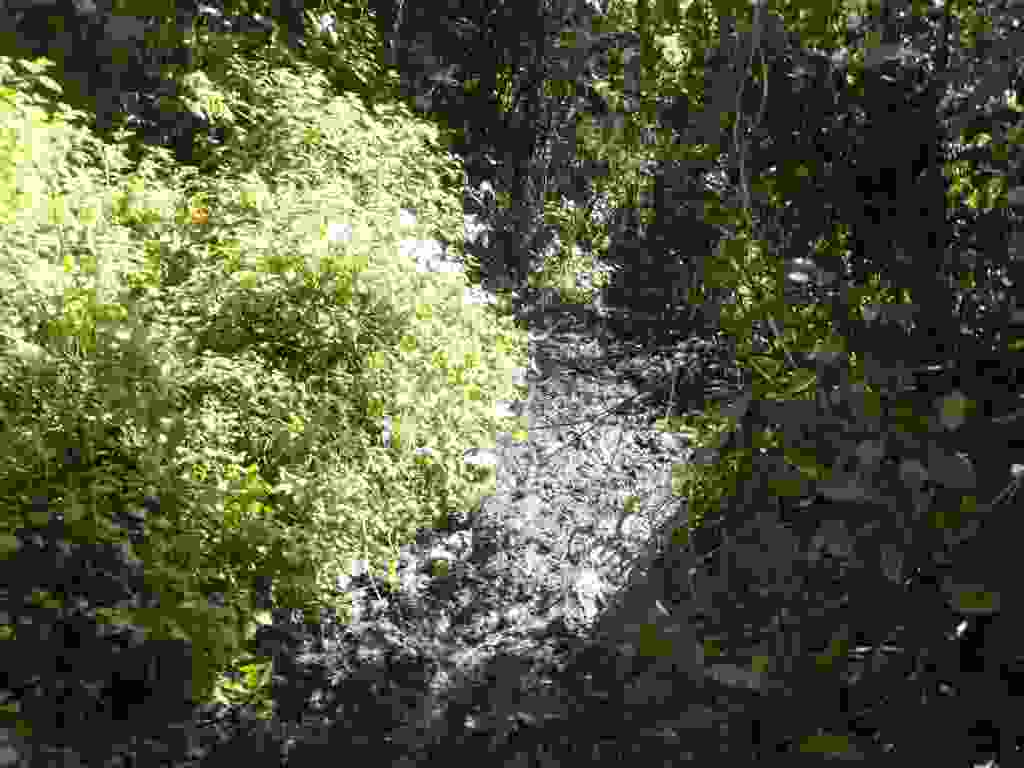
\includegraphics[width=\mywidth]{../wp-content/uploads/2015/06/P6144872-1024x768.jpg} } 
 \newline
 Je prends ensuite la route vers le nord pour une traversée de l´Equateur par les montagnes. \newline
 \newline
\centerline{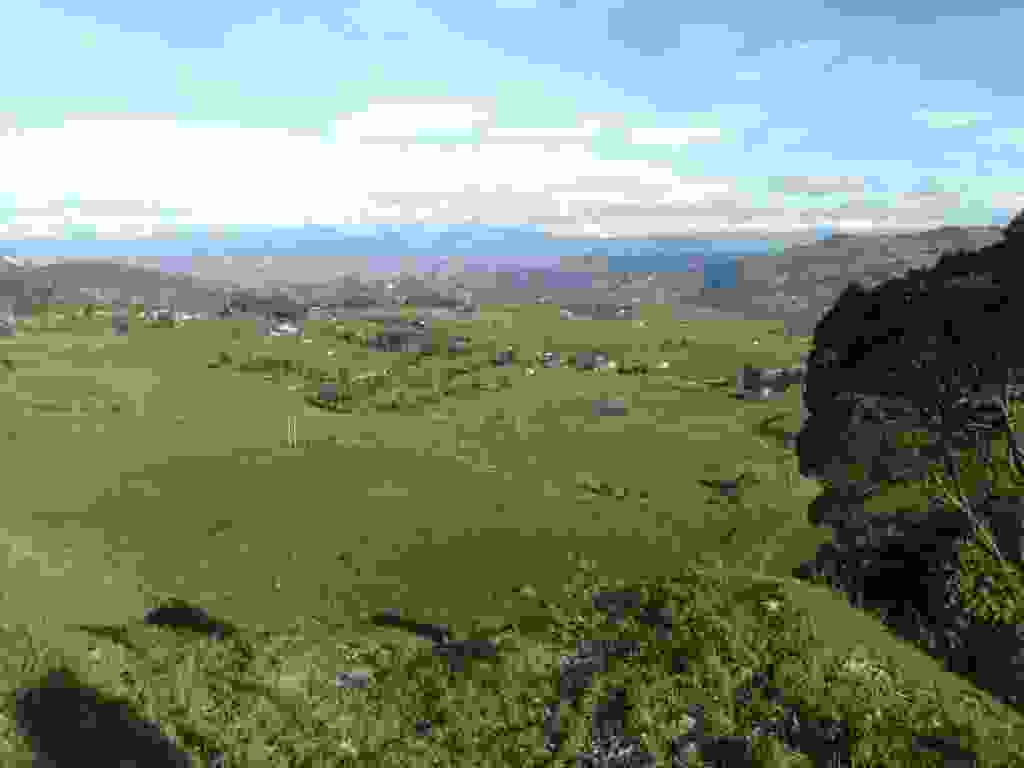
\includegraphics[width=\mywidth]{../wp-content/uploads/2015/06/P6154884-1024x768.jpg} } 
 \newline
 \newline
\centerline{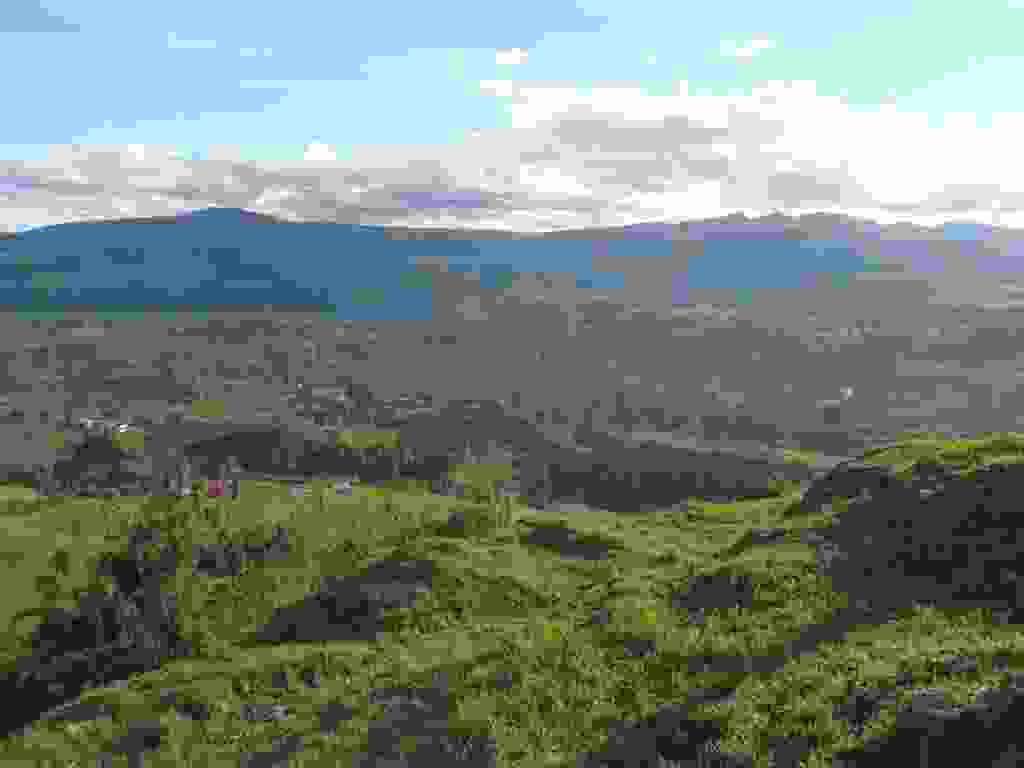
\includegraphics[width=\mywidth]{../wp-content/uploads/2015/06/P6154885-1024x768.jpg} } 
 \newline
 La région est très agricole, je peux observer les cultures associées de maïs et haricots. \newline
 \newline
\centerline{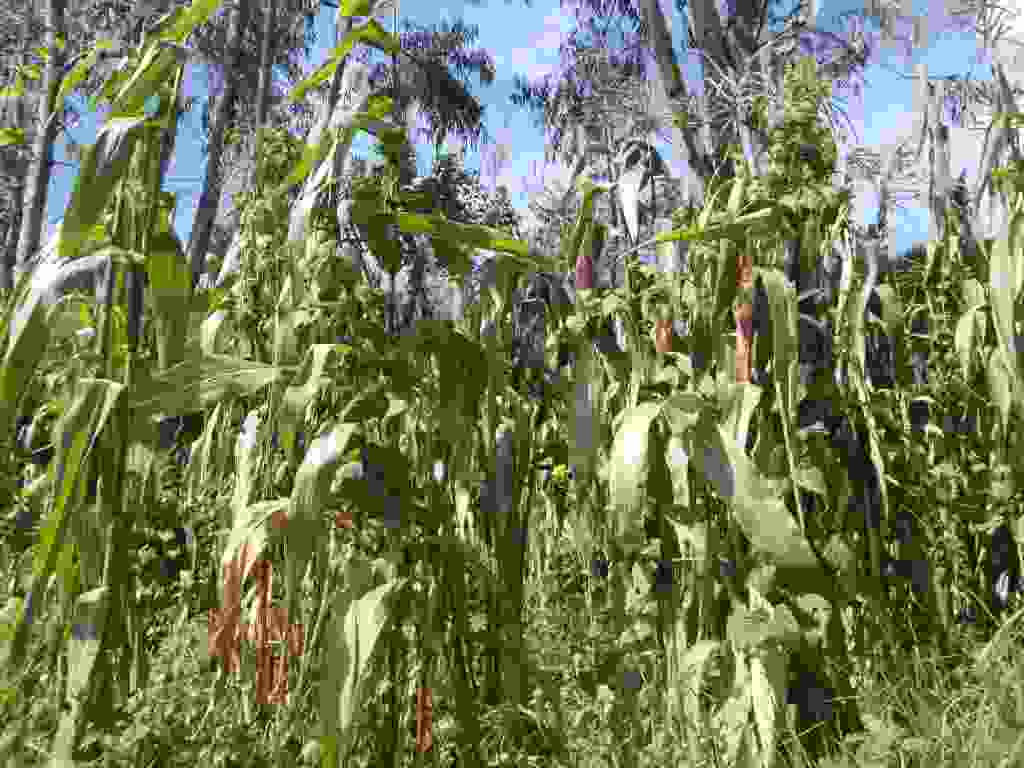
\includegraphics[width=\mywidth]{../wp-content/uploads/2015/06/P6154881-1024x768.jpg} } 
 \newline
 Beaucoup de chiens aussi, l´un d´entre eux a essayé de manger une sacoche arrière, heureusement c´est solide. \newline
 Pause dans le village d´El Tambo. \newline
 \newline
\centerline{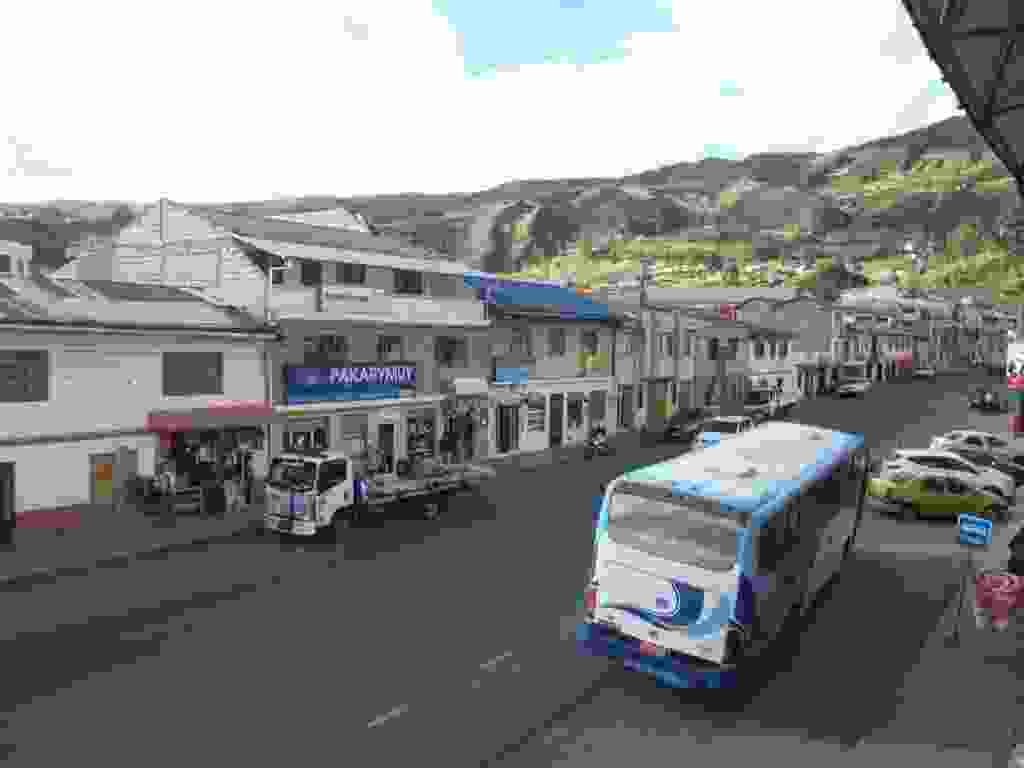
\includegraphics[width=\mywidth]{../wp-content/uploads/2015/06/P6164891-1024x768.jpg} } 
 \newline
 La route continue avec un enchainement de cols, ca monte bien ! \newline
 \newline
\centerline{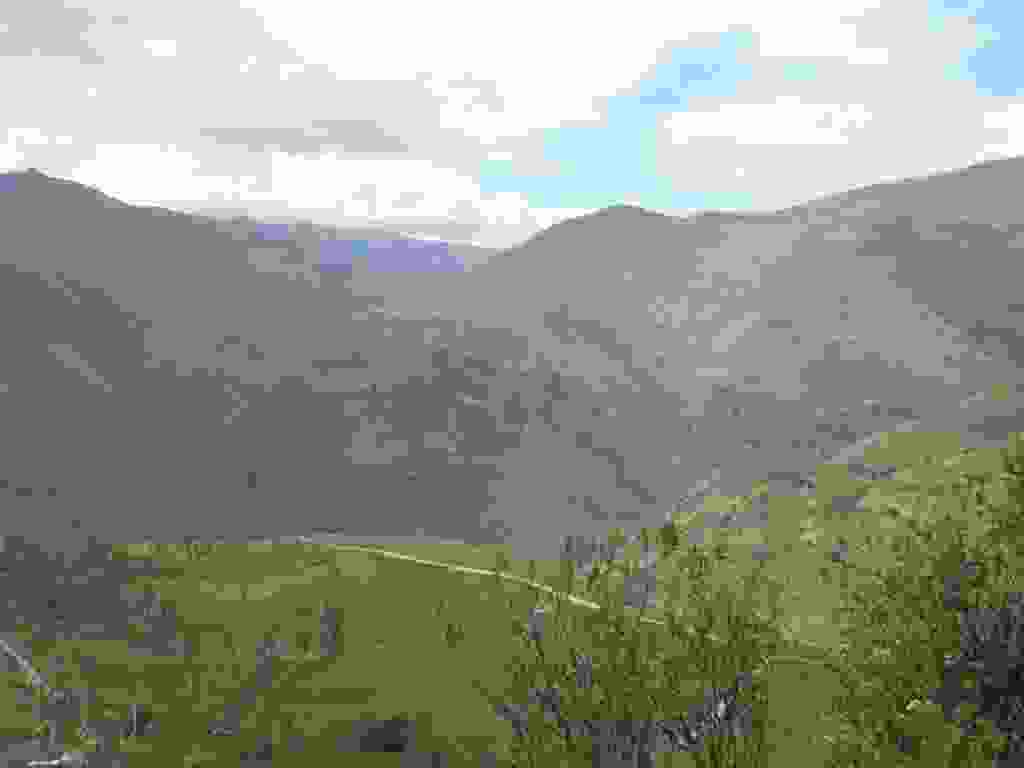
\includegraphics[width=\mywidth]{../wp-content/uploads/2015/06/P6174899-1024x768.jpg} } 
 \newline
 \newline
\centerline{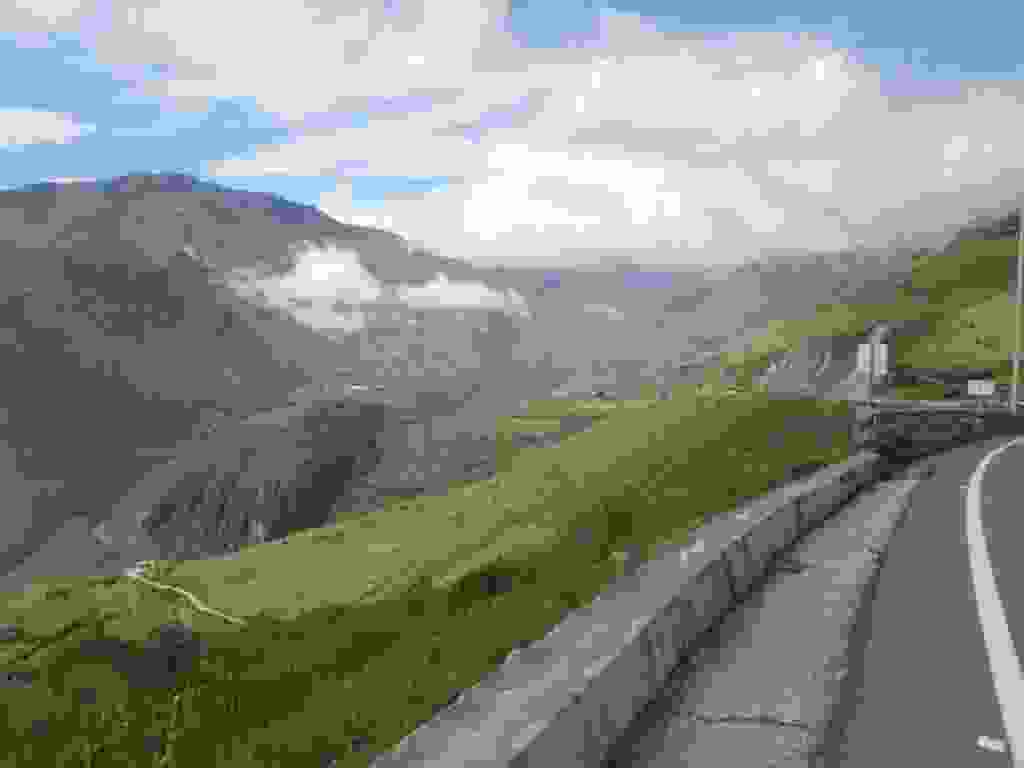
\includegraphics[width=\mywidth]{../wp-content/uploads/2015/06/P6174901-1024x768.jpg} } 
 \newline
 Bivouac au dessus de la petite ville d´Alausi. \newline
 \newline
\centerline{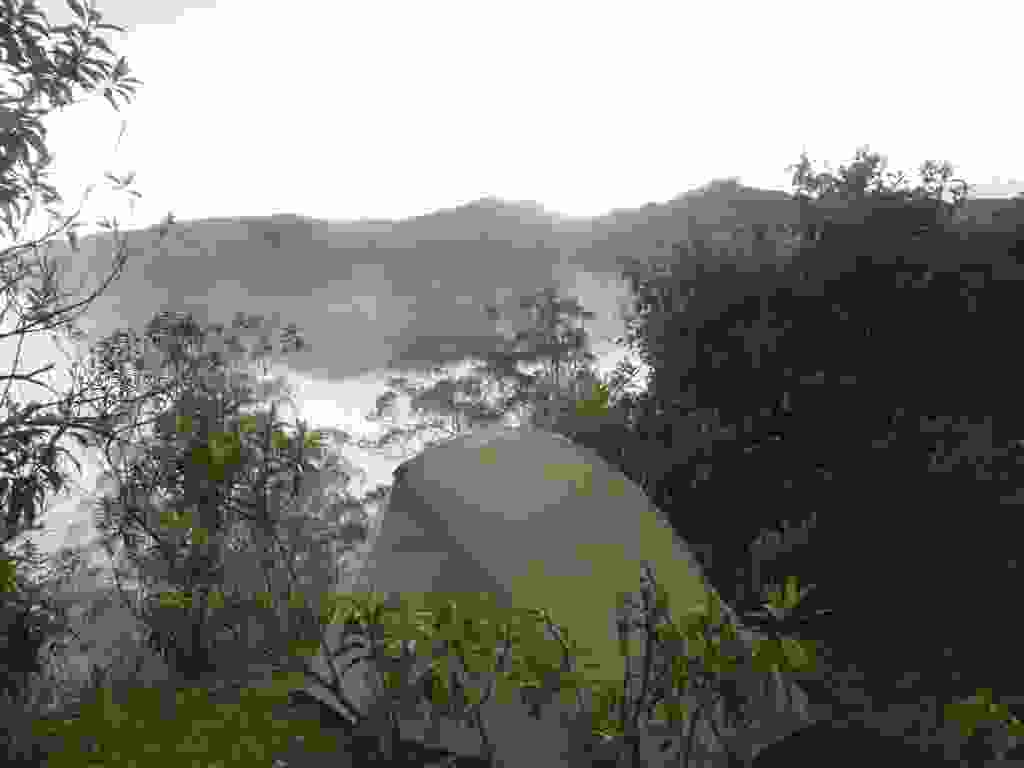
\includegraphics[width=\mywidth]{../wp-content/uploads/2015/06/P6184909-1024x768.jpg} } 
 \newline
 \newline
\centerline{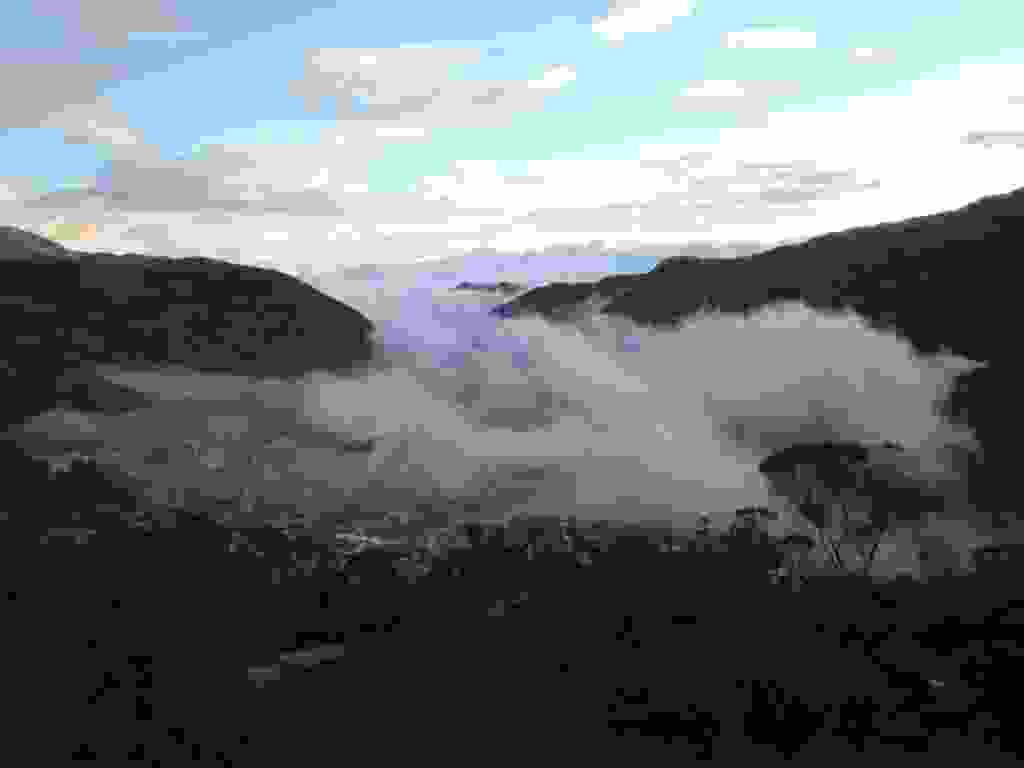
\includegraphics[width=\mywidth]{../wp-content/uploads/2015/06/P6184910-1024x768.jpg} } 
 \newline
 Je m´arrete dans un village pour faire des courses, un jeune me demande d´essayer le vélo. J´hésite mais je le laire faire : l´erreur, après seulement 5m il tombe et casse la béquille du vélo ! Au moins le vélo sera un peu plus léger maintenant… \newline
 Encore des km et du dénivelé avant de passer par Riobamba. \newline
 \newline
\centerline{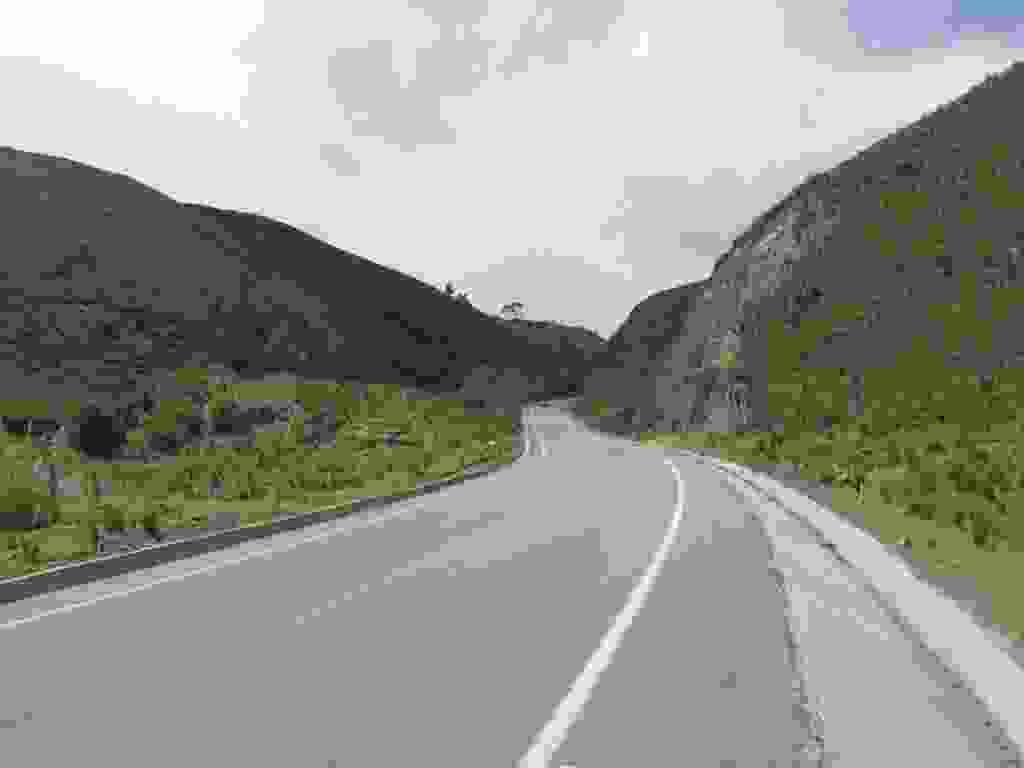
\includegraphics[width=\mywidth]{../wp-content/uploads/2015/06/P6184917-1024x768.jpg} } 
 \newline
 \newline
\centerline{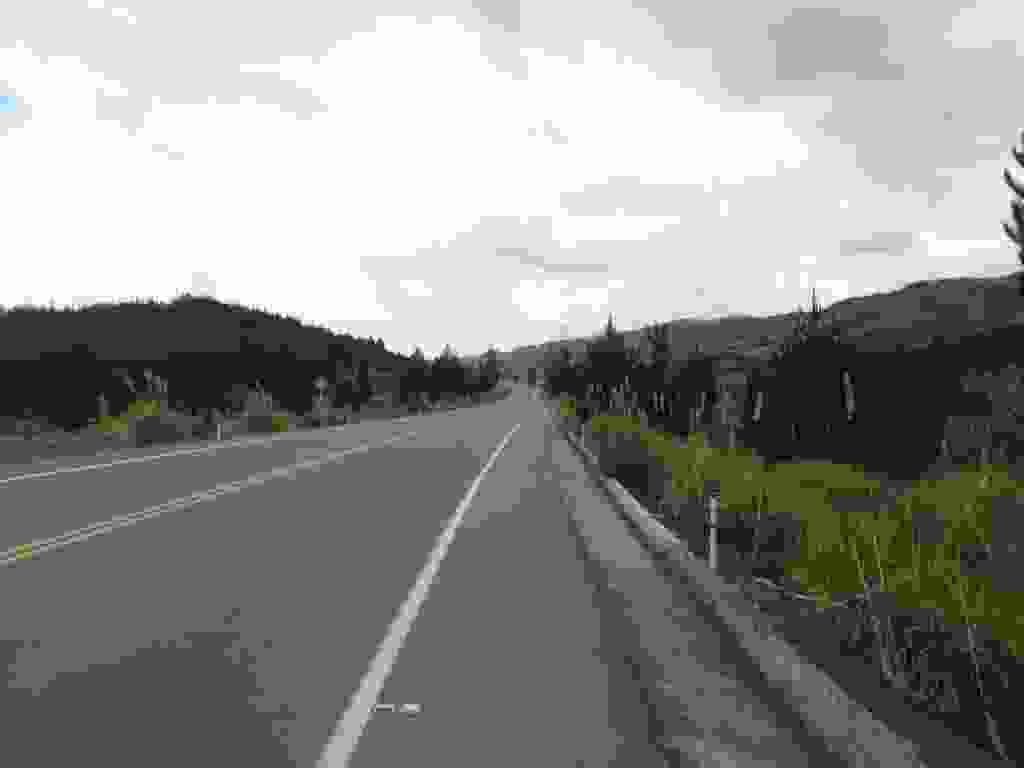
\includegraphics[width=\mywidth]{../wp-content/uploads/2015/06/P6184918-1024x768.jpg} } 
 \newline
 \newline
\centerline{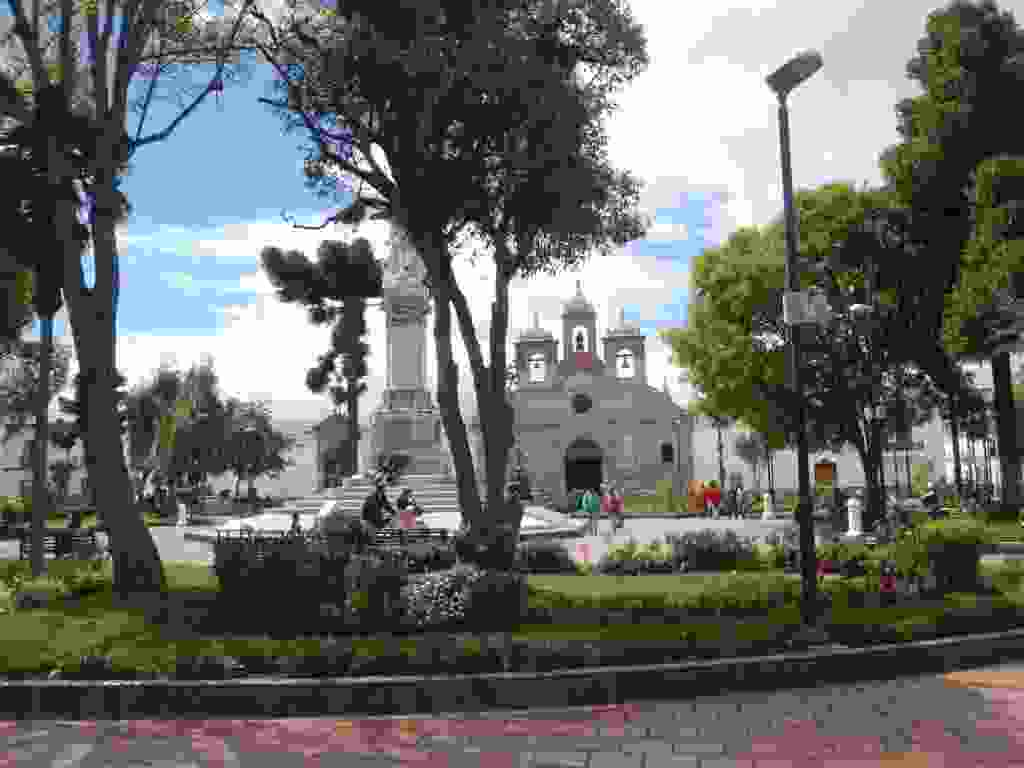
\includegraphics[width=\mywidth]{../wp-content/uploads/2015/06/P6194924-1024x768.jpg} } 
 \newline
 La dernière journée avant Baños est sous la pluie et dans le brouillard, en plus je me trompe de route et je fais un détour de 10km, en montée bien sur ! \newline
 La vue est inexistante mais heureusement des panneaux placés tous les km donnent des conseils écologiques fort utiles. \newline
 \newline
\centerline{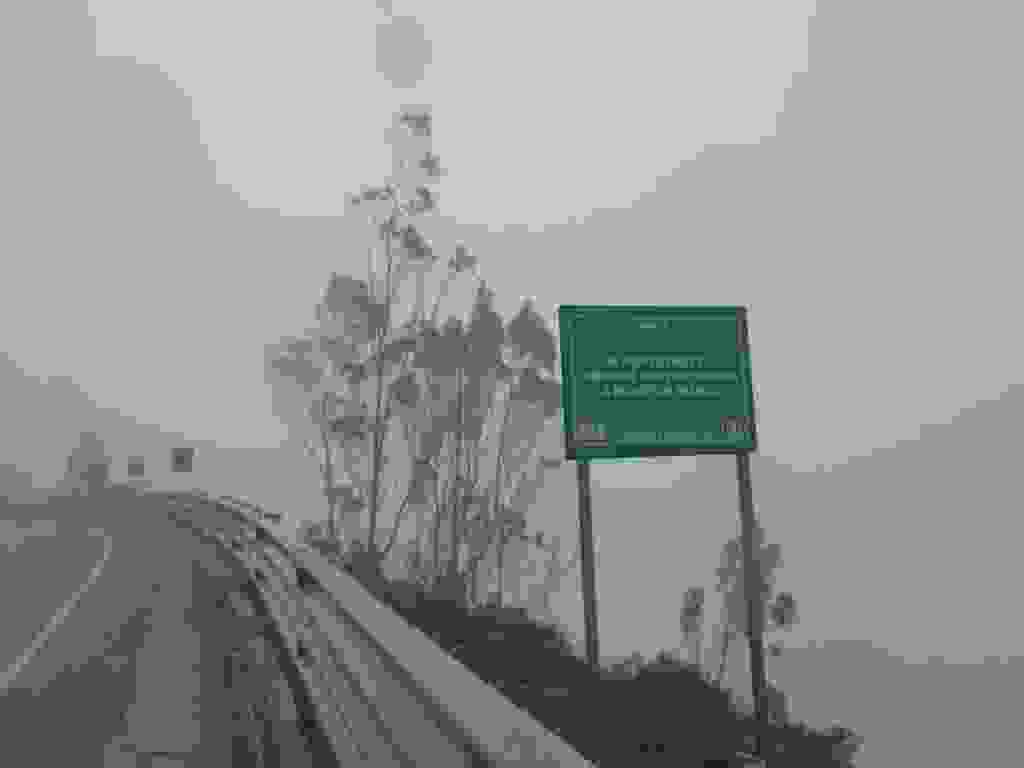
\includegraphics[width=\mywidth]{../wp-content/uploads/2015/06/P6204934-1024x768.jpg} } 
 \newline
 J´arrive enfin à Baños de Agua Santa dans les montagnes, réputée pour ses bains chauds mais surtout pour les activités sportives à proximité : rafting, canyoning, vélo, randonnées… \newline
 \newline
\centerline{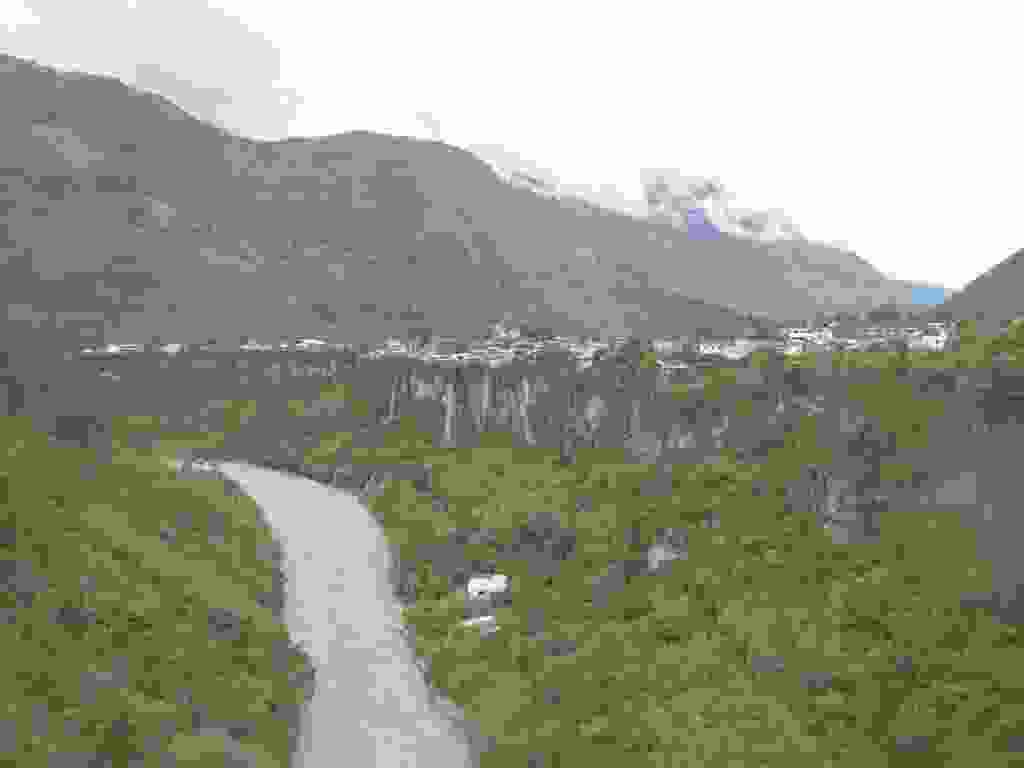
\includegraphics[width=\mywidth]{../wp-content/uploads/2015/06/P6214949-1024x768.jpg} } 
 \newline
 \newline
\centerline{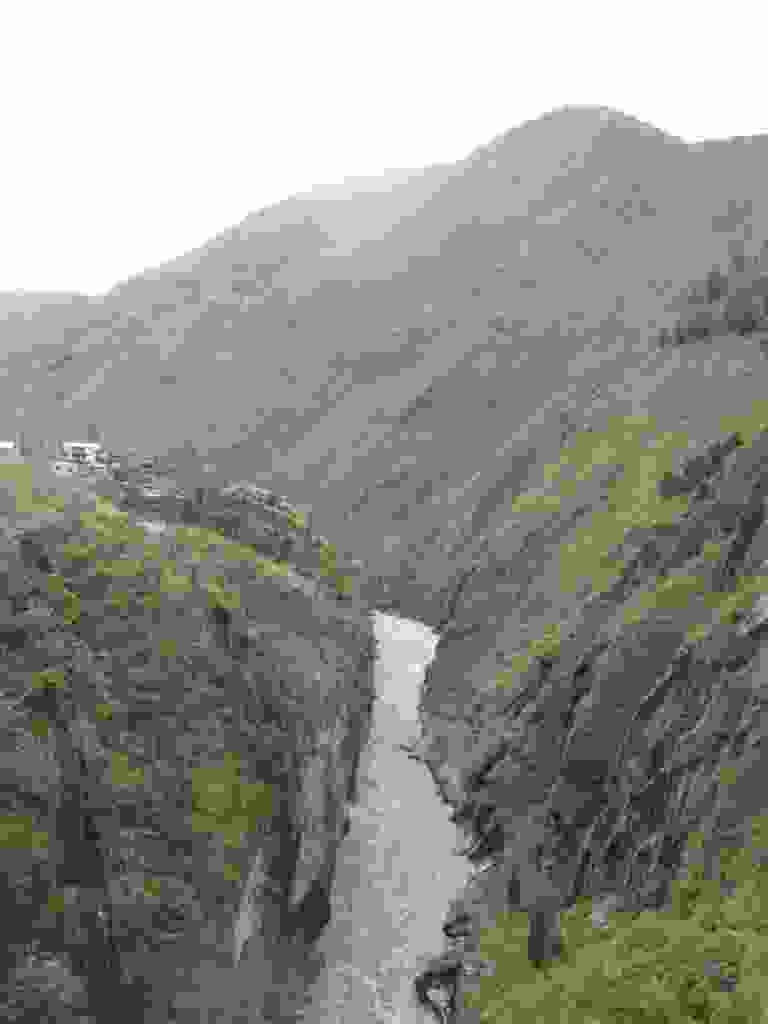
\includegraphics[width=\mywidth]{../wp-content/uploads/2015/06/P6214951-768x1024.jpg} } 
 \newline
 \newline
\centerline{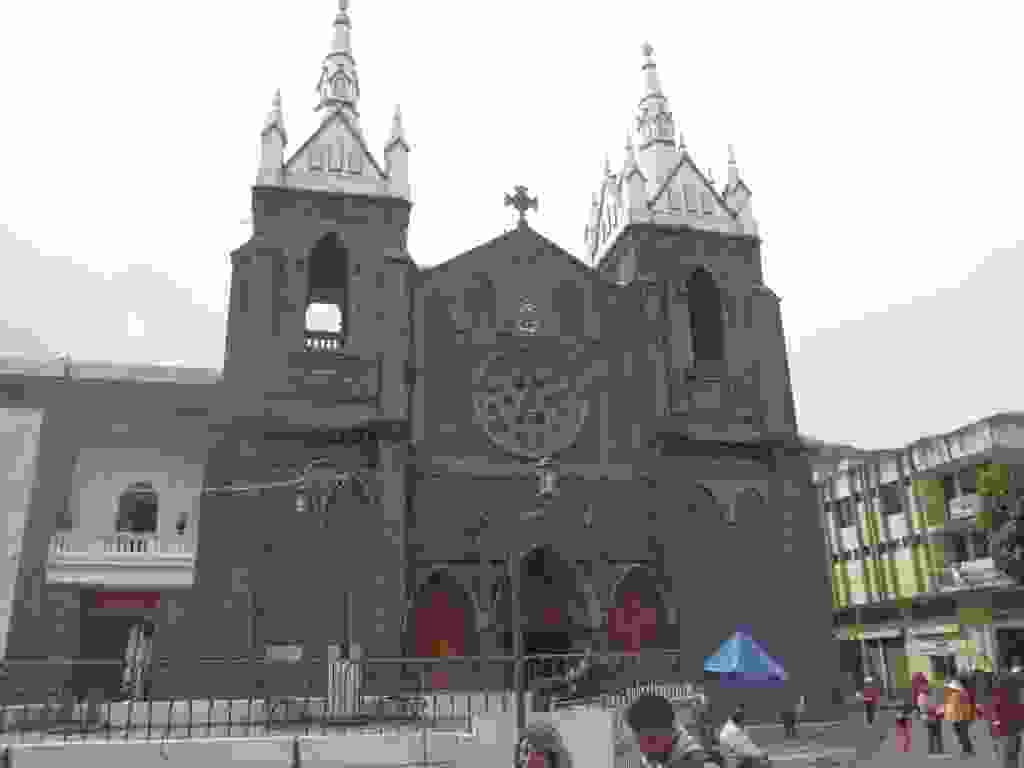
\includegraphics[width=\mywidth]{../wp-content/uploads/2015/06/P6204941-1024x768.jpg} } 
 \newline
 \newline
\centerline{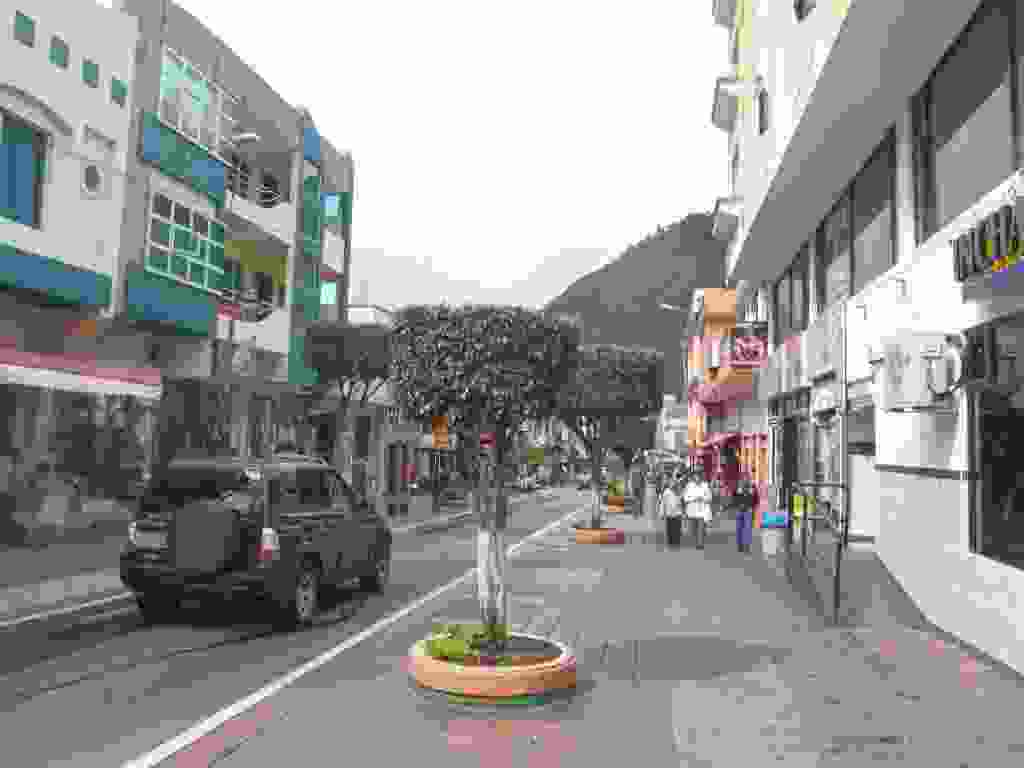
\includegraphics[width=\mywidth]{../wp-content/uploads/2015/06/P6204937-1024x768.jpg} } 
 \newline
 Des stands vendent la canne à sucre sous toutes ses formes. \newline
 \newline
\centerline{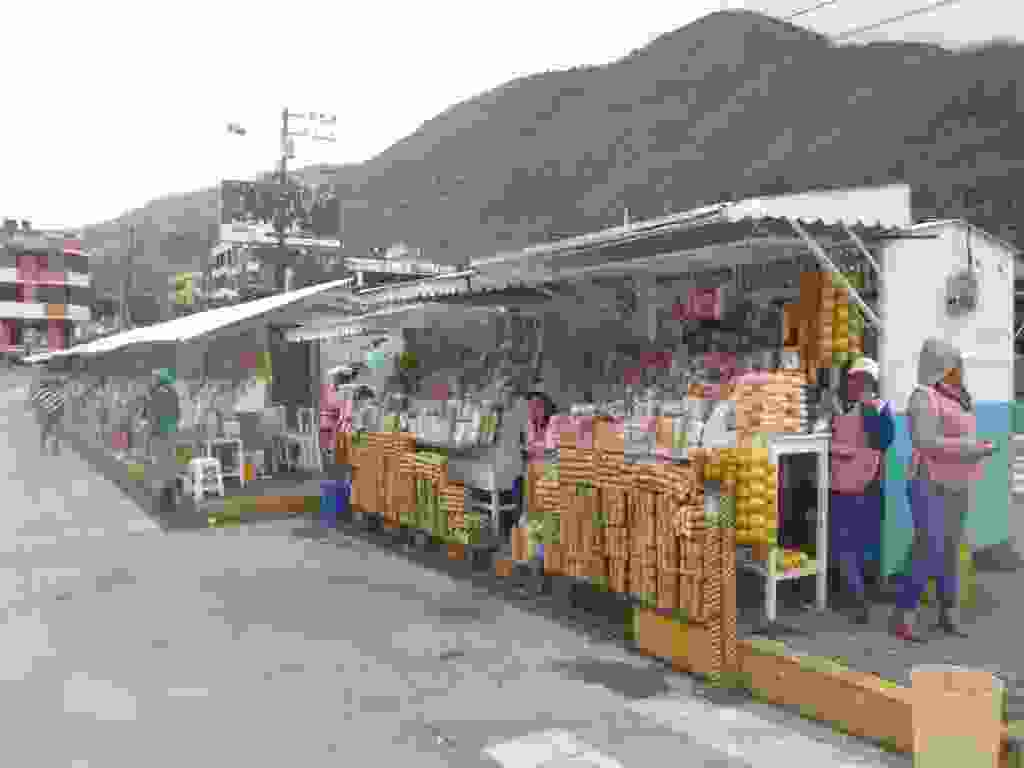
\includegraphics[width=\mywidth]{../wp-content/uploads/2015/06/P6214946-1024x768.jpg} } 
 \newline
 Au dessus de Baños, la Casa de l´Arbol avec parfois une belle vue. \newline
 \newline
\centerline{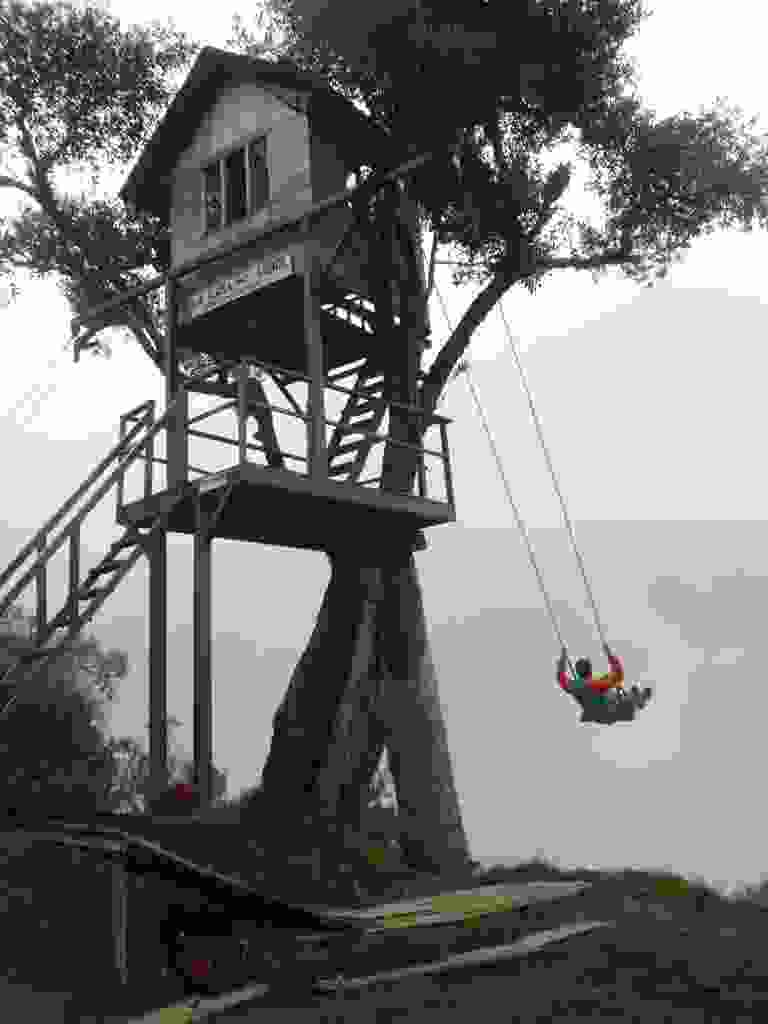
\includegraphics[width=\mywidth]{../wp-content/uploads/2015/06/P6214962-768x1024.jpg} } 
 \newline

\newpage
 
